\documentclass[10pt]{beamer}
\usetheme[
%%% options passed to the outer theme
%    hidetitle,           % hide the (short) title in the sidebar
%    hideauthor,          % hide the (short) author in the sidebar
%    hideinstitute,       % hide the (short) institute in the bottom of the sidebar
%    shownavsym,          % show the navigation symbols
%    width=2cm,           % width of the sidebar (default is 2 cm)
%    hideothersubsections,% hide all subsections but the subsections in the current section
%    hideallsubsections,  % hide all subsections
    left               % right of left position of sidebar (default is right)
%%% options passed to the color theme
%    lightheaderbg,       % use a light header background
  ]{AAUsidebar}

% If you want to change the colors of the various elements in the theme, edit and uncomment the following lines
% Change the bar and sidebar colors:
%\setbeamercolor{AAUsidebar}{fg=red!20,bg=red}
%\setbeamercolor{sidebar}{bg=red!20}
% Change the color of the structural elements:
%\setbeamercolor{structure}{fg=red}
% Change the frame title text color:
%\setbeamercolor{frametitle}{fg=blue}
% Change the normal text color background:
%\setbeamercolor{normal text}{bg=gray!10}
% ... and you can of course change a lot more - see the beamer user manual.


\usepackage[utf8]{inputenc}
\usepackage[english]{babel}
\usepackage[T1]{fontenc}
% Or whatever. Note that the encoding and the font should match. If T1
% does not look nice, try deleting the line with the fontenc.
\usepackage{helvet}

% colored hyperlinks
\newcommand{\chref}[2]{%
  \href{#1}{{\usebeamercolor[bg]{AAUsidebar}#2}}%
}


\date{\today}


	\title{sw608f14 - Piktotegner}
	\author{Daniel S. F, Lars A, Mathias W. P. \& Søren S. A.}
% - Give the names in the same order as they appear in the paper.
% - Use the \inst{?} command only if the authors have different
%   affiliation. See the beamer manual for an example

\institute[
%  {\includegraphics[scale=0.2]{aau_segl}}\\ %insert a company, department or university logo
  Dept.\ of Computer Science\\
  Aalborg University\\
  Denmark
] % optional - is placed in the bottom of the sidebar on every slide
{% is placed on the title page
  Department of Computer Science\\
  Aalborg University\\
  Denmark
  
  %there must be an empty line above this line - otherwise some unwanted space is added between the university and the country (I do not know why;( )
}


% specify a logo on the titlepage (you can specify additional logos an include them in 
% institute command below
\pgfdeclareimage[height=1.5cm]{titlepagelogo}{AAUgraphics/aau_logo_new} % placed on the title page
%\pgfdeclareimage[height=1.5cm]{titlepagelogo2}{graphics/aau_logo_new} % placed on the title page
\titlegraphic{% is placed on the bottom of the title page
  \pgfuseimage{titlepagelogo}
%  \hspace{1cm}\pgfuseimage{titlepagelogo2}
}


\begin{document}
% the titlepage
{\aauwavesbg%
\begin{frame}[plain,noframenumbering] % the plain option removes the sidebar and header from the title page
  \titlepage
\end{frame}}
%%%%%%%%%%%%%%%%

% TOC
\begin{frame}{Agenda}{}
\tableofcontents
\end{frame}
%%%%%%%%%%%%%%%%
	
	
	\section{Multi Project}
	\begin{frame}
	\frametitle{Multi Project}
		\begin{itemize}
		\item GIRAF
		\item Large Setting
		\item SCRUM
		\item Tools
		\item Specialists
		\end{itemize}
		More slides may be added for each item here.
	\end{frame}
	
	
	\section{Old Piktotegner}
		\begin{frame}
		\frametitle{Old Piktotegner}
		\begin{figure}
			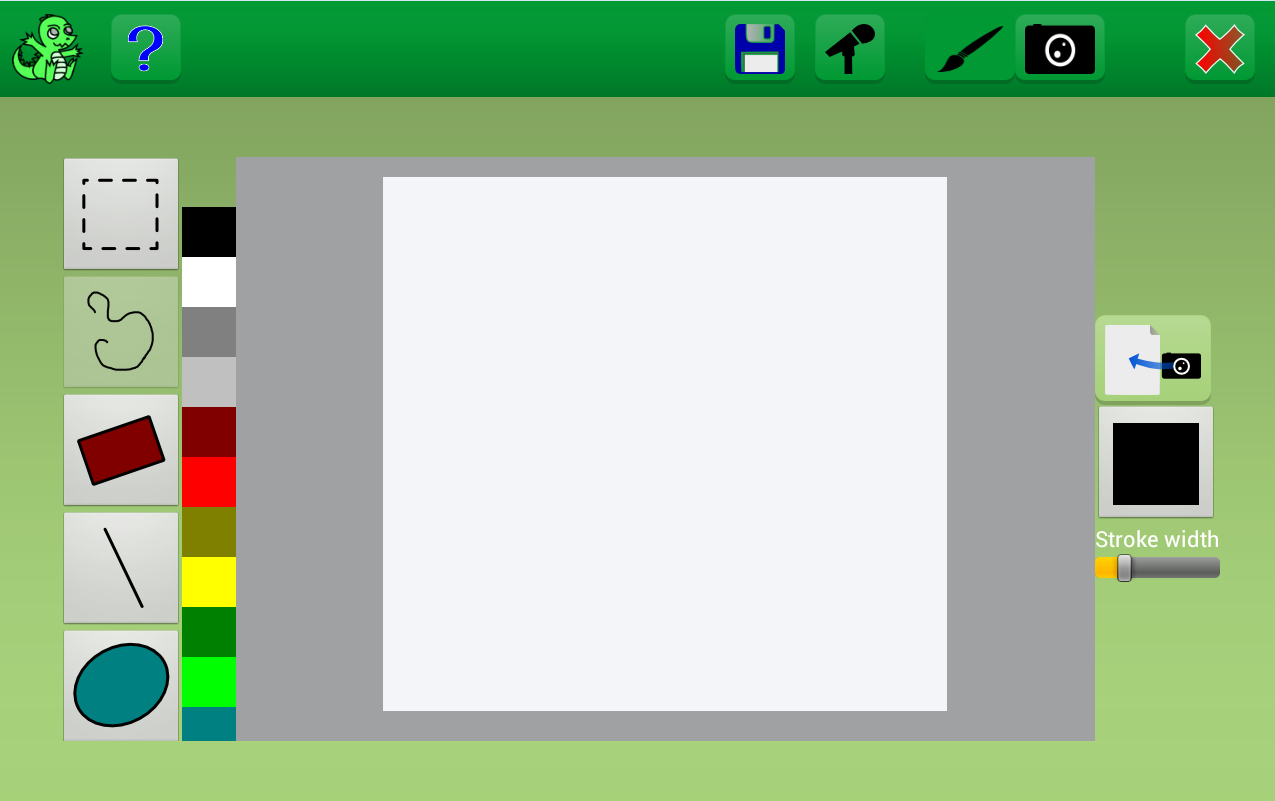
\includegraphics[width=\textwidth]{media/CrocOldCanvas}
			\caption{Old Piktotegner Layout}
		\end{figure}
		\end{frame}
	
	\section{Key Changes}
	\begin{frame}
	\frametitle{Key Changes}
		Each key changes listed here will have slides for that given change. Before and after pictures will be shown for this.
		\begin{itemize}
		\item Rotation
		\item Resize
		\item Collision detection
		\item Recording audio
		\item Saving and loading for piktograms
		\item Camera
		\end{itemize}
	\end{frame}
	
	\section{Usability test}
		\begin{frame}
		\frametitle{Usability test}
		\begin{itemize}
			\item Why?
			\item How?
			\item Results
		\end{itemize}
	
		\end{frame}
	
	\section{Media Library Collaboration}
		\begin{frame}
		\frametitle{Media Library Collaboration}
		\begin{itemize}
			\item MediaPlayer
			\item Text to Speech
			\item Collaboration experience
		\end{itemize}

		\end{frame}
		
	\section{Demonstration}
	
		\begin{frame}
		\frametitle{Demonstration}
		Here use an emulator to present the developed product, or preferably with a tablet.
			\begin{figure}
				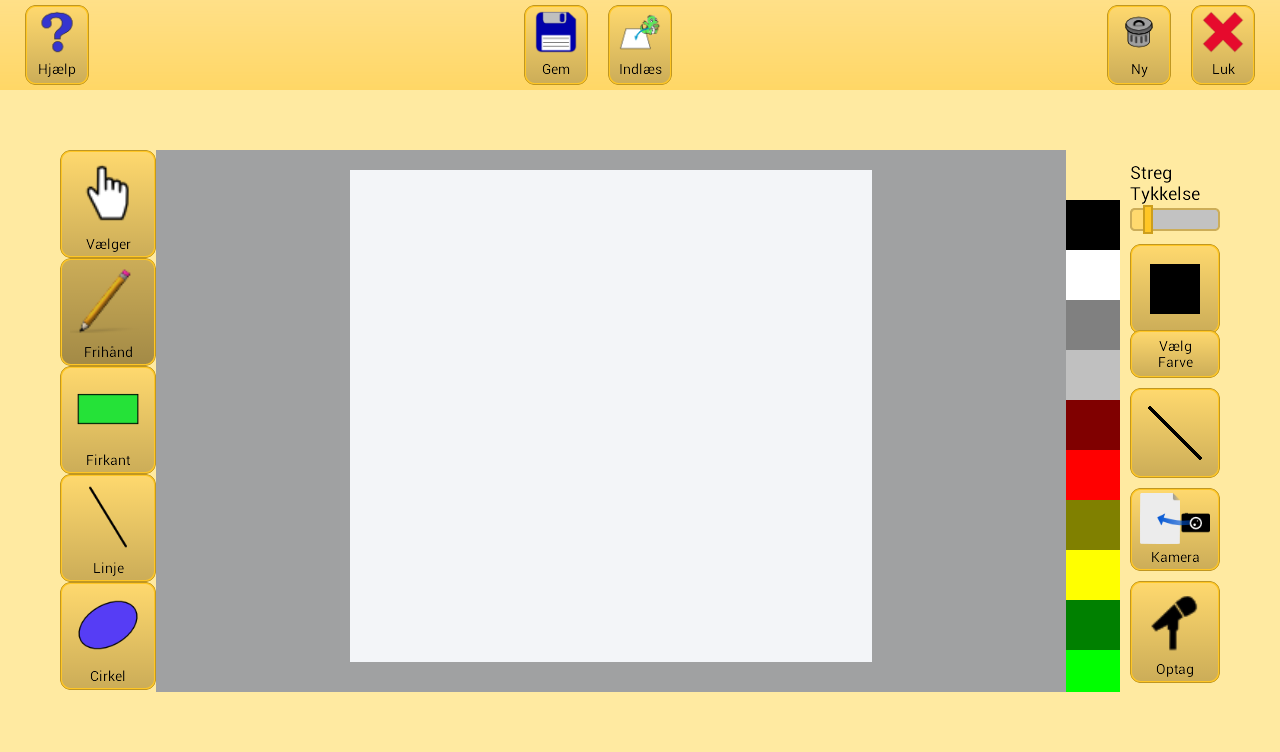
\includegraphics[width=\textwidth]{media/final-main-ui}
				\caption{New Piktotegner Layout}
			\end{figure}
		\end{frame}		

	\section{Reflections}
		\begin{frame}
		\frametitle{Reflections}
		\begin{itemize}
			\item Usability test experience gain
			\item SCRUM experience
			\item Customer interaction
			\item Further Development
		\end{itemize}
		More points to be added
		\end{frame}


	\bgroup
	\setbeamercolor{background canvas}{bg=black}
	\begin{frame}[plain]{}
	\addtocounter{framenumber}{-1}	
		\begin{center}
		%\textcolor{white}{END}
		\end{center}
	\end{frame}
	\egroup
\end{document}
